\chapter{Iteración II - Agente de Imitación}
\label{chap:iter2}

\lettrine{E}{sta} iteración aborda el aprendizaje por imitación (\gls{il}), entrenando
una \gls{política} que reproduce el comportamiento del experto simbólico a partir del
conjunto de demostraciones generado en la iteración anterior (Sección~\ref{sec:dataset-htn}, página~\pageref{sec:dataset-htn}).

Para mostrar la evolución del agente, se realiza una explicación
de las iteraciones realizadas durante el desarrollo del modelo de imitación: desde una primera
versión que aprende solo del estado, pasando por la adición de la visión y la
limitación de tratar la cámara como acciones discretas, hasta la arquitectura final
de doble cabeza.

Como resultado se obtiene un agente de imitación que consigue realizar la tarea de
\gls{woodcutting}. Sin la información privilegiada de la \acrshort{api}, el agente aprende
a orientarse hacia el tronco y atacarlo. Si bien no presenta una fase de exploración
consistente (Sección~\ref{sec:il-sin-exploracion}, página~\pageref{sec:il-sin-exploracion}),
la política aprendida sí que consigue el objetivo de la tarea bajo condiciones favorables.

\section{Motivación}
A diferencia del agente \gls{htn} (Capítulo~\ref{chap:iter1}), que decide a partir de la información de la \acrshort{api}, el agente de imitación debe aprender a actuar
a partir de la información que le presenta el experto. En este caso: la imagen del
visor en primera persona y un pequeño vector de estado, con información que el jugador podría obtener
fácilmente, como su cambio de posición o si lo que está viendo es un tronco.

El \textit{dataset} utilizado para el entrenamiento consta de un total de 
\num{118} episodios y \num{4094} pares \textit{OBSERVACIÓN-ACCIÓN} (\num{4069} tras la limpieza), cada
uno con la estructura descrita en la Tabla~\ref{tab:dataset-frame}
(página~\pageref{tab:dataset-frame}). 
El problema principal encontrado a la hora de realizar el entrenamiento
es el propio experto: como ya se vio en la Figura~\ref{fig:dataset-clases}
(página~\pageref{fig:dataset-clases}), la distribución de acciones está
fuertemente desbalanceada, ya que el experto solo ejecuta unas pocas de las
acciones disponibles. Sus causas y su tratamiento se abordan en la
Sección~\ref{sec:desbalanceo} (página~\pageref{sec:desbalanceo}).

\section{Entrenamiento sobre el Dataset}
En esta sección se describen las decisiones de diseño al procesar el \textit{dataset} de 
demostraciones y los parámetros utilizados en el entrenamiento.

\subsection{Fuga de Datos}
Como los \textit{frames} de un mismo episodio son muy
similares entre sí, una partición aleatoria del \textit{dataset} filtraría información
del conjunto de \textit{test} al de entrenamiento, contaminando al modelo. La
división del conjunto se hace, entonces, por sesión: episodios completos van a
entrenamiento o a \textit{test}, nunca repartidos. Esto garantiza que la validación
mide la capacidad de generalizar en episodios no vistos.

\subsection{Tratamiento del Desbalanceo}
\label{sec:desbalanceo}
Para el tratamiento del desbalanceo de clase observado en el \textit{dataset} (Figura~\ref{fig:dataset-clases}, página~\pageref{fig:dataset-clases}),
se aplican las tres técnicas mostradas a continuación. Si bien estos tratamientos podrían eliminar información del experto,
lo que se intenta con ellos es que el modelo aprenda un comportamiento realista usando como referencia al experto:

\begin{itemize}
  \item \textbf{Pesos por clase balanceados}: las acciones
  minoritarias pesan más durante el entrenamiento. Dado que la acción dominante 
  \textit{attack} representa el \qty{70}{\percent} de los \textit{frames},
  su contribución al gradiente se reduce para que el modelo no aprenda a predecirla siempre.
  \item \textbf{Descarte de clases poco representadas}: el \gls{htn}
  navega de forma tan óptima con el \gls{pathfinder} que el \textit{dataset} apenas contiene
  cuatro de las nueve acciones discretas. El filtro descarta además las clases con
  menos muestras que un umbral (p.\ ej., \textit{jump}, con solo \num{25} apariciones de \num{4094} \textit{frames}),
  que no aportan ejemplos suficientes para un comportamiento real, de modo que el
  espacio discreto queda reducido a tres clases (\textit{attack},
  \textit{move\_forward\_sprint} y \textit{move\_forward\_jump}).
  \item \textbf{Aumento de datos (\textit{Data Augmentation})}: las imágenes del entorno son simétricas. Dadas las tres acciones consideradas,
  su imagen correspondiente es la misma que su versión volteada horizontalmente. Esto lo podemos aprovechar
  para duplicar el \textit{dataset}: se invierte la imagen del visor, se intercambian
  las etiquetas \textit{move\_left}$\leftrightarrow$\textit{move\_right} y se invierte
  el signo de $\Delta\text{\textit{yaw}}$.
\end{itemize}

\subsection{Hiperparámetros}
Como optimizador se utiliza \textit{AdamW}
(\textit{lr}=\num{e-4}, \textit{weight\_decay}=\num{e-2}), un planificador
\textit{ReduceLROnPlateau} que reduce el \textit{learning rate} al estancarse la
pérdida de validación, y \textit{early stopping} sobre la precisión de validación.

Además, en la normalización de la cámara, los
$\Delta\text{\textit{yaw}}$ y $\Delta\text{\textit{pitch}}$ se acotan a $\pm\num{1}$~rad antes de normalizar,
eliminando giros bruscos ($>\num{1}$~rad) que son generados por el \gls{pathfinder} y
que no buscamos que el modelo reproduzca. La Tabla~\ref{tab:il-hparams} (página~\pageref{tab:il-hparams}) resume la
configuración:

\begin{table}[htbp]
  \centering
  \resizebox{\textwidth}{!}{%
  \small
  \rowcolors{2}{white}{udcgray!25}
  \begin{tabular}{l|l}
  \rowcolor{udcpink!25}
  \textbf{Hiperparámetro} & \textbf{Valor} \\\hline
  Longitud de secuencia ($T$)   & \num{4} \textit{frames} \\
  Optimizador                   & \textit{AdamW} (\textit{lr}=\num{e-4}, \textit{weight\_decay}=\num{e-2}) \\
  Planificador de \textit{lr}   & \textit{ReduceLROnPlateau} (factor \num{0.5}, \textit{min\_lr}=\num{e-6}) \\
  Pérdida de acción             & \textit{CrossEntropyLoss} (pesos balanceados, \textit{label smoothing}) \\
  Pérdida de cámara             & \textit{MSELoss} \\
  Tamaño de \textit{batch}      & \num{32} \\
  Partición \textit{train}/\textit{val} & por sesión (evita fuga temporal) \\
  Regularización                & \textit{dropout} (\num{0.5} acción, \num{0.3} cámara), \textit{weight decay}, \textit{early stopping} \\
  Aumentado                     & Volteo horizontal con intercambio de etiquetas \\
  \end{tabular}
  }
  \caption[Configuración de entrenamiento del agente de imitación]{Configuración de entrenamiento del agente \gls{il}.}
  \label{tab:il-hparams}
\end{table}

\section{Implementación de Solo Estado}
\label{sec:solo-estado}
Las primeras versiones del agente intentan simular la percepción de la versión simbólica.
Si bien el agente de la primera iteración presenta una imitación de visión usando el \gls{fov},
no es una visión real como la que tendría un jugador, con la capacidad de ver literalmente los bloques, árboles, etc.
Por ello, la primera iteración utiliza únicamente el vector de estado que, eliminando el componente de visión,
es lo más cercano a la información que tendría el experto que podemos obtener.

Con ello se utiliza una \textbf{única cabeza de clasificación}, 
mostrada en la Figura~\ref{fig:il-arch-state} (página~\pageref{fig:il-arch-state}),
sobre un espacio de acciones discretas,
donde el modelo recibe como entrada únicamente el vector de estado. 
Esta versión \textit{limitada} permite generar
una cota inferior de referencia para próximas versiones.
Cualquier modelo visual posterior debe, como mínimo, igualar lo que se obtiene con
esta versión simple.

\begin{figure}[htbp]
  \centering
  \resizebox{\textwidth}{!}{%
  \begin{tikzpicture}[
    font=\footnotesize, >=Latex, node distance=6mm,
    box/.style ={draw, rounded corners, align=center, minimum height=8mm, minimum width=20mm},
    inp/.style ={draw, rounded corners, align=center, fill=udcgray!20, minimum height=8mm},
    tmp/.style ={box, fill=orange!12},
    headc/.style={box, fill=green!12},
    outn/.style ={box, fill=udcgray!20},
  ]
    \node[inp]  (st)   {Estado $T{\times}4$};
    \node[box, fill=udcgray!10] (proj) [right=10mm of st] {\textit{Linear}\\$6\!\to\! d$};
    \node[tmp]  (lstm) [right=10mm of proj] {\textit{lstm}\\$d\!\to\!256$};
    \node[headc] (ah)  [right=10mm of lstm] {\textit{action\_head}\\\scriptsize Dropout$\to$Linear};
    \node[outn] (ao)   [right=8mm of ah] {acción\\discreta};

    \draw[->] (st)   -- (proj);
    \draw[->] (proj) -- (lstm);
    \draw[->] (lstm) -- (ah);
    \draw[->] (ah)   -- (ao);
  \end{tikzpicture}
  }
  \caption[Arquitectura de la variante solo-estado]{Arquitectura de la variante
  solo estado: el vector de estado sirve de entrada a la red \gls{lstm} y una
  única cabeza de clasificación predice la acción discreta. La variable $d$ es la 
  dimensión del espacio de características.
  Sin entrada visual ni cabeza de cámara, es la base sobre la que las variantes siguientes añaden el
  extractor visual y la segunda cabeza (Figura~\ref{fig:il-arch-dual}, página~\pageref{fig:il-arch-dual}).}
  \label{fig:il-arch-state}
\end{figure}

El vector de estado consta de \num{6} componentes normalizadas a $[-\num{1},\num{1}]$ mediante
\emph{cotas fijas} conocidas del entorno\footnote{Rangos máximos de la cámara, máxima distancia posible entre posiciones
de un \textit{frame} a otro, distancia máxima hacia un árbol.}: orientación de cámara
(\textit{yaw}, \textit{pitch}), movimiento respecto al \textit{frame} anterior
($\Delta x, \Delta z$) y dos señales de percepción obtenidas a través del \gls{fov}
(\textit{tree\_visible}, \textit{tree\_distance}). Se excluye la posición absoluta
($x, y, z$) ya que con coordenadas absolutas la red puede tender a memorizar posiciones
del mundo en lugar de generalizar; el movimiento útil se encuentra en $\Delta x, \Delta z$.
La red presenta un componente temporal ($T=\num{4}$ \textit{frames}), ya que las acciones se benefician 
de la información contextual a lo largo del tiempo.
Si el agente se encuentra atacando, es probable que en el siguiente \textit{frame} siga atacando,
o si se encuentra moviéndose hacia el tronco,
es probable que siga moviéndose hacia él.

La salida del modelo es, entonces, la mejor acción a realizar dado un entorno.
Estas acciones recogen las acciones de movimiento, ataque y ocho acciones de cámara que aplican giros fijos de $\pm\ang{15}$ y
$\pm\ang{45}$ en \textit{yaw} y \textit{pitch}, hasta sumar \num{17} acciones en total.

Observando la Tabla~\ref{tab:il-eval} (página~\pageref{tab:il-eval}), la variante solo-estado
alcanza una tasa de éxito del \qty{4}{\percent} (recoger $k=\num{5}$ troncos), con una media ($\mu$) de \num{0.54} troncos por episodio y
una mediana ($\tilde{x}$) de \num{0.00}. Esto indica la incapacidad del agente para aprender a realizar la tarea de forma
ciega y muestra la necesidad de incorporar la entrada visual. 
Se refuerza con la Figura~\ref{fig:il-action-dist} (página~\pageref{fig:il-action-dist}),
donde se observa que el agente realiza la acción de ataque el \qty{99.3}{\percent} de las veces. Al estar en un entorno
rodeado de troncos, el agente aprende a atacar constantemente, pero es incapaz de orientarse o
saber si es capaz de romperlos.

\section{Incorporación de la Entrada Visual}
Como se menciona en la sección anterior, en la variante solo-estado el agente es incapaz de orientarse hacia un tronco,
ya que desconoce la posición real del mismo.
La segunda versión incorpora la \textbf{imagen del visor} (Apéndice~\ref{apx:frame}) sumada al vector de estado.
Esto proporciona al modelo gran parte de la información que un jugador humano tendría,
permitiendo al agente aprender a orientarse hacia el tronco y atacarlo, sin cruzar la línea
de la omnisciencia, como sería usar el \gls{pathfinder} de la versión simbólica (Capítulo~\ref{chap:iter1}).
Se ilustra la arquitectura de la variante visual de una cabeza en la Figura~\ref{fig:camara-discreta} (página~\pageref{fig:camara-discreta}).


\begin{figure}[htbp]
  \centering
  \resizebox{\textwidth}{!}{
  \begin{tikzpicture}[
    font=\footnotesize, >=Latex, node distance=6mm,
    box/.style ={draw, rounded corners, align=center, minimum height=8mm, minimum width=20mm},
    inp/.style ={draw, rounded corners, align=center, fill=udcgray!20, minimum height=8mm},
    ext/.style ={box, fill=blue!8},
    fus/.style ={draw, circle, inner sep=1pt, minimum size=5mm},
    tmp/.style ={box, fill=orange!12},
    headc/.style={box, fill=green!12},
    outn/.style ={align=center},
  ]
    \node[inp] (img)   {Imagen $T{\times}4$\\(visor 1ª pers.)};
    \node[inp] (st)    [below=10mm of img] {Estado $T{\times}4$\\\scriptsize(pos, cámara, percepción)};

    \node[ext] (extr)  [right=10mm of img]  {Extractor\\visual};
    \node[box, fill=udcgray!10] (proj) [right=10mm of st] {\textit{Linear}\\$\to d$};

    \node[fus] (sum)   at ($(extr)!0.5!(proj) + (16mm,0)$) {$+$};
    \node[tmp] (lstm)  [right=8mm of sum] {\gls{lstm}\\$d\!\to\!256$};

    \node[headc] (ah)  [right=10mm of lstm] {\textit{head}\\\scriptsize Dropout$\to$Linear};
    \node[outn] (ao)   [right=9mm of ah] {$17$ acciones\\\scriptsize $9$ mov./ataque\\$+\,8$ cámara discretas};

    \draw[->] (img)  -- (extr);
    \draw[->] (st)   -- (proj);
    \draw[->] (extr) -- (sum);
    \draw[->] (proj) -- (sum);
    \draw[->] (sum)  -- (lstm);
    \draw[->] (lstm) -- (ah);
    \draw[->] (ah)   -- (ao);
  \end{tikzpicture}
  }
  \caption[Arquitectura de cabeza única (cámara discreta)]{Arquitectura de cabeza
  única: la imagen y el estado se fusionan por suma, pasan por la \gls{lstm} y
  una \emph{única} cabeza de clasificación elige una de \num{17} acciones discretas, de
  las cuales \num{8} son giros de cámara fijos ($\pm\ang{15}$, $\pm\ang{45}$). Al ser
  mutuamente excluyentes, el agente no puede girar la cámara y desplazarse en el
  mismo paso; esta limitación motiva la doble cabeza (Figura~\ref{fig:il-arch-dual}, página~\pageref{fig:il-arch-dual}).}
  \label{fig:camara-discreta}
\end{figure}

La imagen de entrada se redimensiona a $\num{128}\times\num{128}$ y se normaliza usando
los valores de media y desviación típica del \textit{dataset} \textit{ImageNet}, ya que uno de los
extractores visuales utilizados es un modelo preentrenado con este conjunto de datos~\cite{DBLP:conf/cvpr/DengDSLL009}.
Un \textbf{extractor} produce un vector de características por \textit{frame} de la imagen del visor que se
fusiona con el estado mediante una suma, cuyo resultado alimenta a la red final
\gls{lstm} (Figura~\ref{fig:il-arch-dual}, página~\pageref{fig:il-arch-dual}).
La salida final es una acción que ejecutará el agente, ya sea moverse, atacar o girar la cámara.

El principal cambio entre las variantes visuales es el extractor, cuya selección final se aborda
en la Sección~\ref{sec:il-extractor} (página~\pageref{sec:il-extractor}). 
Cabe mencionar que una de las variantes, aparte de modificar el extractor,
cambia la red troncal por una \gls{convlstm} en lugar de una \gls{lstm}\footnote{A lo largo del
capítulo se referenciará la ConvLSTM como un extractor más por conveniencia.}.
Para el vector de estado se realiza una proyección lineal a un espacio de características de la misma dimensión que el 
extractor visual, para permitir la suma de los vectores.
A diferencia de la concatenación, la suma mantiene la entrada a la \gls{lstm} en un tamaño fijo $d$
independientemente de si hay imagen o no, de modo que las variantes solo-estado y
visual comparten exactamente la misma arquitectura. Además, al usar la suma, el tamaño del vector resultante 
es menor al de la concatenación; provocando una leve mejora en el coste de entrenamiento. 

Por último, la red troncal empleada es una \gls{lstm} con \num{256} unidades ocultas,
seleccionada por su capacidad de aprender dependencias temporales. Como ya se señaló en la
Sección~\ref{sec:solo-estado} (página~\pageref{sec:solo-estado}), las acciones no son independientes entre sí, por lo que se
mantiene el \textit{\gls{frame-stacking}} ($T=\num{4}$ \textit{frames}) para aportar contexto temporal.


\subsection{Cámara como Acciones Discretas y su Limitación}
\label{sec:il-camara-discreta}
El modelo simbólico era capaz de realizar múltiples acciones a la vez
(moverse/atacar y mover la cámara simultáneamente).
Pero con el diseño de una sola cabeza las acciones son mutuamente excluyentes (una por \textit{frame});
mover la cámara y avanzar o atacar no
pueden ocurrir a la vez. En la práctica el experto sí ajusta la cámara mientras se
acerca al tronco, de modo que la información de cámara se perdía en todos los
\textit{frames} con una acción de movimiento o ataque.

A esta limitación se añade que las ocho clases de cámara, con apenas \numrange{5}{39}
muestras cada una, caían constantemente bajo el umbral de \textit{min\_samples}
y se eliminaban del entrenamiento.
Si el agente mueve la cámara \ang{15} en \num{5} de cada \num{4094} \textit{frames} de entrenamiento,
no es un comportamiento a aprender, sino ruido para el modelo.

El modelo de cabeza única alcanzaba una precisión de acción superior
(\qty{92.5}{\percent}), como recoge la Tabla~\ref{tab:single-vs-dual} (página~\pageref{tab:single-vs-dual}), pero solo
porque la tarea quedaba reducida a un problema binario (\textit{attack} frente a \textit{move\_forward\_sprint}) 
en el que el agente no aprendía a orientar la cámara en absoluto.

Estas limitaciones motivan la arquitectura final, donde el agente predice la cámara con relación
a la acción que tiene que ejecutar, pudiendo dejar la cámara sin mover con un $\Delta\text{\textit{yaw}}=\num{0}$ y $\Delta\text{\textit{pitch}}=\num{0}$.

\begin{table}[htbp]
  \centering
  \resizebox{\textwidth}{!}{
  \rowcolors{2}{white}{udcgray!25}
  \begin{tabular}{l|c|c|l}    
  \rowcolor{udcpink!25}
  \rowcolor{udcpink!25}
  \textbf{Modelo} & \textbf{Acc. acción (\%)} & \textbf{Clases} & \textbf{Cámara} \\\hline
  Cabeza única & \num{92.5} & \num{2} & \num{8} clases discretas, eliminadas en limpieza \\
  Cabeza dual        & \num{77.3} & \num{3} & Continua (regresión $\Delta\text{\textit{yaw}}, \Delta\text{\textit{pitch}}$) \\
  \end{tabular}
  }
  \caption[Cabeza única frente a cabeza dual]{Comparación de la cabeza única
  (cámara discreta) frente a la doble cabeza. La mayor precisión de la cabeza única
  es engañosa: solo conserva dos clases de acción porque descarta toda la
  cámara; la doble cabeza conserva las acciones disponibles del experto y, además, modela el movimiento
  de cámara continuo.}
  \label{tab:single-vs-dual}
\end{table}

\subsection{Implementación de la Cabeza Dual}
\label{sec:il-arch-dual}

La solución al problema de la cámara consiste en separar el movimiento de cámara del resto de acciones, 
de modo que la cámara deje de competir con ellas y pase a registrarse
y predecirse en cada \textit{frame} como una variable separada.
El nuevo espacio de control pasa a ser: una acción discreta y un movimiento de cámara continuo
($\Delta\text{\textit{yaw}}, \Delta\text{\textit{pitch}}$, resultante del movimiento de un \textit{frame} a otro).
La arquitectura resultante se observa en la Figura~\ref{fig:il-arch-dual} (página~\pageref{fig:il-arch-dual}).
A continuación se describen las dos cabezas de la arquitectura final:

\begin{figure}[htbp]
  \centering
  \resizebox{\textwidth}{!}{
  \begin{tikzpicture}[
    font=\footnotesize, >=Latex, node distance=6mm,
    box/.style ={draw, rounded corners, align=center, minimum height=8mm, minimum width=18mm},
    inp/.style ={draw, rounded corners, align=center, fill=udcgray!20, minimum height=8mm},
    ext/.style ={box, fill=blue!8},
    fus/.style ={draw, circle, inner sep=1pt, minimum size=5mm},
    tmp/.style ={box, fill=orange!12},
    headc/.style={box, fill=green!12},
    headr/.style={box, fill=red!10},
    outn/.style ={align=center},
  ]
    \node[inp] (img)   {Imagen $T{\times}$6\\(visor 1ª pers.)};
    \node[inp] (st)    [below=8mm of img] {Estado $T{\times}6$\\\scriptsize(cámara, $\Delta$, percepción)};

    \node[ext] (extr)  [right=8mm of img]  {Extractor\\visual};
    \node[box, fill=udcgray!10] (proj) [right=8mm of st] {\textit{Linear}\\$6\!\to\! d$};

    \node[fus] (sum)   at ($(extr)!0.5!(proj) + (12mm,0)$) {$+$};
    \node[tmp] (lstm)  [right=6mm of sum] {\gls{lstm}\\$d\!\to\!256$};

    % Reorientación: ramas arriba y abajo
    \node[headc] (ah)  [above right=6mm and 8mm of lstm.east] {\textit{action\_head}\\\scriptsize Dropout$\to$Linear};
    \node[headr] (ch)  [below right=6mm and 8mm of lstm.east] {\textit{camera\_head}\\\scriptsize Dropout$\to$Linear$\to\tanh$};

    \node[outn] (ao)    [right=6mm of ah] {acción\\discreta};
    \node[outn] (co)    [right=6mm of ch] {$(\Delta\text{\textit{yaw}},\Delta\text{\textit{pitch}})$};

    \draw[->] (img)  -- (extr);
    \draw[->] (st)   -- (proj);
    \draw[->] (extr) -- (sum);
    \draw[->] (proj) -- (sum);
    \draw[->] (sum)  -- (lstm);
    \draw[->] (lstm.east) -- (ah.west);
    \draw[->] (lstm.east) -- (ch.west);
    \draw[->] (ah)   -- (ao);
    \draw[->] (ch)   -- (co);
  \end{tikzpicture}
  }
  \caption[Arquitectura de doble cabeza del agente de imitación]{Arquitectura final
  de doble cabeza. Las características visuales y el estado proyectado se
  suman, pasando a una red \gls{lstm} que aporta contexto temporal y dos cabezas de salida para la predicción de:  
  la acción discreta (clasificación) y el desplazamiento de cámara continuo
  (regresión con $\tanh$).}
  \label{fig:il-arch-dual}
\end{figure}

\begin{itemize}
  \item \textbf{Cabeza de clasificación} (\textit{action\_head}): dado el estado y
  las características visuales, predice la acción correspondiente.
  \item \textbf{Cabeza de regresión} (\textit{camera\_head}): predice
  $(\Delta\text{\textit{yaw}}, \Delta\text{\textit{pitch}})$ con una activación $\tanh$ que acota la
  salida a $[-\num{1},\num{1}]$, el mismo rango al que se normalizan en
  el entrenamiento. Luego se desnormaliza a radianes en inferencia para el control del agente
  y, además, se descartan los giros bruscos ($>\num{1}$~rad) que el \gls{pathfinder} del \gls{htn} introduce de
  forma puntual.
\end{itemize}

Cada cabeza tiene su propia función de pérdida; la cabeza de acción utiliza la función
\textit{CrossEntropyLoss} con pesos balanceados y \textit{label smoothing}, 
mientras que la cabeza de cámara usa \textit{MSELoss}. La función de pérdida total de la red
se calcula como la suma de ambas pérdidas:
\begin{equation}
  \mathcal{L} = \mathcal{L}_{\text{acción}} + \mathcal{L}_{\text{cámara}}
\end{equation}
    
\section{Selección del Extractor Visual}
\label{sec:il-extractor}
Una vez fijada la arquitectura de doble cabeza, es necesario seleccionar el mejor extractor visual 
para la red. Se evaluaron tres alternativas, recogidas en la Tabla~\ref{tab:progresion-il} (página~\pageref{tab:progresion-il}), 
todas bajo la misma configuración (misma partición de datos, mismos hiperparámetros):

\begin{itemize}
  \item \gls{gru}: trata cada fila de la imagen como
  una secuencia, procesando la imagen de arriba abajo. Se eligió usar una \gls{gru} frente a una \gls{rnn}
  clásica tras compararlas en igualdad de condiciones: la \gls{gru} alcanzó
  un \qty{77.3}{\percent} frente al \qty{66.9}{\percent} de la \gls{rnn} (\num{10.4} puntos de ventaja).
  \item \gls{convlstm}: combina una \gls{cnn} con una celda
  recurrente convolucional. Con esta arquitectura, se pretendía ver si la parte más significativa
  de la arquitectura era el extractor visual o la red troncal.
  \item \gls{vit}: preentrenado en \textit{ImageNet}. El modelo utilizado fue
  adaptado a entradas de $\num{128}\times\num{128}$ (\num{64} \textit{\glspl{token}} de $\num{16}\times\num{16}$).
\end{itemize}

\begin{table}[htbp]
  \centering
  \resizebox{\textwidth}{!}{
  \small
  \rowcolors{2}{white}{udcgray!25}
  \begin{tabular}{l|c|c|c}
  \rowcolor{udcpink!25}
  \textbf{Variante} & \textbf{Acc. validación (\%)} & \textbf{Loss acción} & \textbf{MSE cámara} \\\hline
  Solo estado & \num{69.4} & \num{0.749} & \num{0.1087} \\
  Visual (GRU) & \num{77.3} & \num{1.193} & \num{0.1251} \\
  Visual (ConvLSTM) & \num{74.7} & \num{0.839} & \num{0.1257} \\
  Visual (ViT) & \num{73.2} & \num{0.865} & \num{0.1322} \\
  \end{tabular}
  }
  \caption[Comparación de extractores visuales]{Comparación de los extractores visuales evaluados en la iteración.
  La variante solo-estado sirve de referencia para la mejora que aporta la entrada visual. Como resultado, 
  la \gls{gru} obtiene la mayor precisión de acción (\qty{77.3}{\percent}) y se selecciona como extractor final.}
  \label{tab:progresion-il}
\end{table}

Lo primero que se observa en la Tabla~\ref{tab:progresion-il} (página~\pageref{tab:progresion-il}) es que la entrada visual mejora la
precisión frente al solo-estado, aumentando la precisión de acción en \num{8} puntos (del \qty{69.4}{\percent} al \qty{77.3}{\percent})
respecto al mejor modelo, lo que confirma que la imagen aporta información que el vector de estado
no captura. Entre los extractores, la \gls{gru} obtiene el mejor resultado
(\qty{77.3}{\percent}), por delante de la \gls{convlstm} (\qty{74.7}{\percent}) y del \gls{vit} (\qty{73.2}{\percent}).

Sin embargo, como se puede observar en la Figura~\ref{fig:il-training} (página~\pageref{fig:il-training}), se aprecia
un claro ejemplo de \gls{overfitting}: el modelo alcanza una gran precisión de entrenamiento ($\sim\qty{97}{\percent}$)
pero no generaliza tan bien al conjunto de validación (\qty{77.3}{\percent}). Esta tendencia se repite en todos
los extractores, especialmente en el \gls{vit} que, a pesar de ser el más pesado y preentrenado, 
es el que más sufre este fenómeno. Las curvas de entrenamiento del resto de modelos se pueden
ver en el Apéndice~\ref{apx:il-curvas}.

\begin{figure}[htbp]
  \centering
  \resizebox{\textwidth}{!}{
  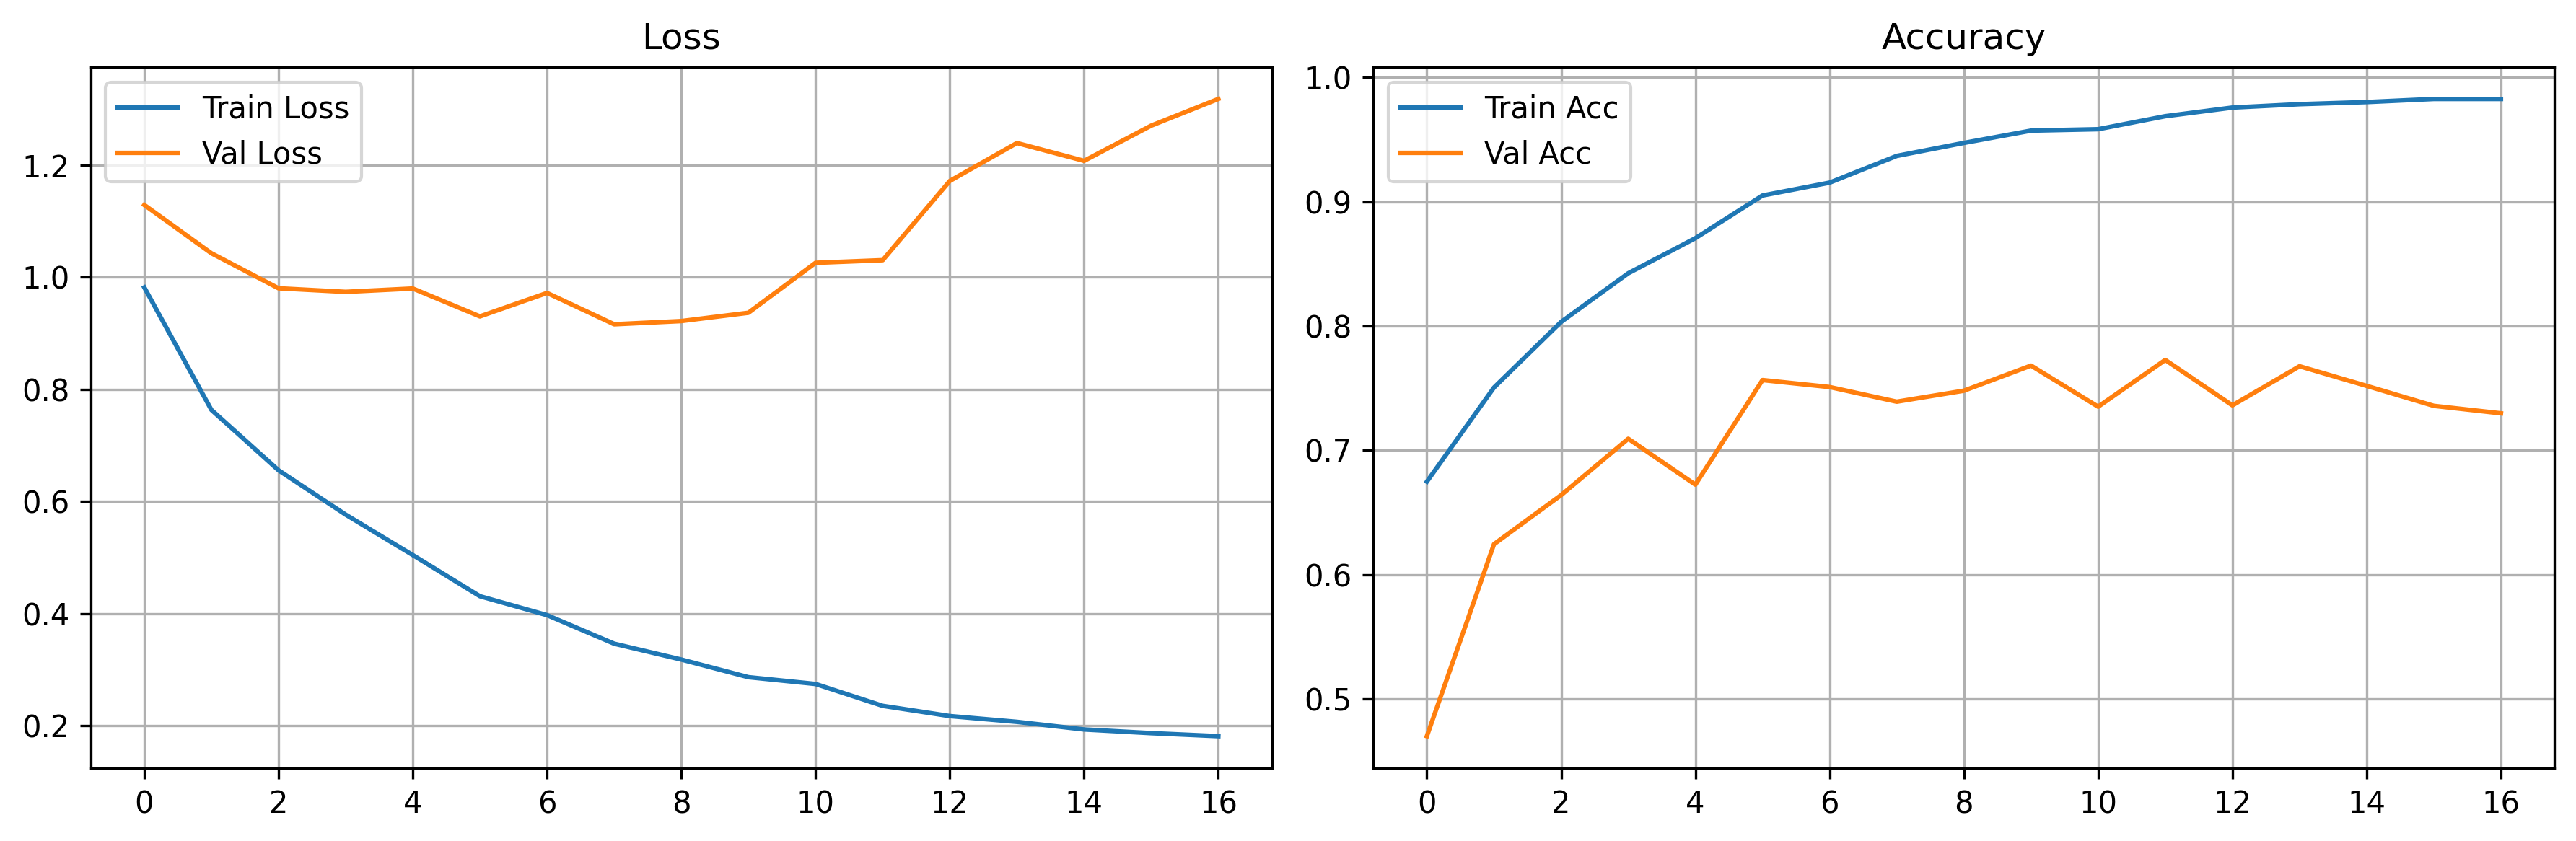
\includegraphics[width=1\textwidth]{imaxes/07_il/il_training_history.png}
  }
  \caption[Curvas de entrenamiento de los extractores visuales]{Evolución de la
  precisión y la pérdida (entrenamiento y validación) del modelo \gls{gru} de doble
  cabeza. La precisión de validación alcanza el \qty{77.3}{\percent}; el \textit{early stopping}
  detiene el entrenamiento al estancarse la mejora.}
  \label{fig:il-training}
\end{figure}


Además, las redes empleadas son considerablemente pequeñas,
como muestra la Tabla~\ref{tab:il-extractores-inferencia}
(página~\pageref{tab:il-extractores-inferencia}): la \gls{convlstm}
es la más ligera (\num{0.38}\,M de parámetros), pero queda \num{2.6} puntos por debajo de la
\gls{gru}. El \gls{vit} es el más pesado (\num{22.2}\,M, de los cuales solo quedan
\num{0.63}\,M entrenables) tras congelar las capas y, sin embargo, es el peor en
precisión. La \gls{gru} ofrece el mejor compromiso entre coste y precisión: con
\num{3.75}\,M de parámetros y sin preentrenamiento, alcanza la
mayor precisión. Esto la convierte en el modelo ganador de la iteración.

\begin{table}[htbp]
  \centering
  \resizebox{\textwidth}{!}{
  \small
  \rowcolors{2}{white}{udcgray!25}
  \begin{tabular}{l|c|c|c} 
  \rowcolor{udcpink!25}
  \textbf{Extractor} & \textbf{Parámetros} & \textbf{Preentrenamiento} & \textbf{Acc. val. (\%)} \\\hline
  \gls{gru} & \num{3.75}\,M            & No            & \textbf{\num{77.3}} \\
  \gls{convlstm}      & \num{0.38}\,M            & No            & \num{74.7} \\
  \gls{vit}    & \num{22.2}\,M \scriptsize(\num{0.63}\,M entrenables) & Sí (\textit{ImageNet}) & \num{73.2} \\
  \end{tabular}
  }
  \caption[Comparación de extractores visuales]{Comparación de tamaño de los tres
  extractores. El \gls{vit} mantiene su \gls{backbone} congelado y solo entrena la cabeza de clasificación, 
  mientras que la \gls{gru} y la \gls{convlstm} se entrenan desde cero.}
  \label{tab:il-extractores-inferencia}
\end{table}

Observando la matriz de confusión (Figura~\ref{fig:il-confusion}, página~\pageref{fig:il-confusion}) se puede apreciar de dónde provienen los errores del modelo. Las acciones \textit{attack} y \textit{move\_forward\_sprint} son las que más seguridad tienen, con un \qty{77.0}{\percent} y un \qty{91.0}{\percent} respectivamente. El principal problema
se encuentra en la acción de \textit{move\_forward\_jump}. Esto se debe a que, para un mismo \textit{frame} y estado, las acciones \textit{move\_forward\_jump} y \textit{move\_forward\_sprint} son muy similares.
Presentan diferencias sutiles, lo que provoca que el modelo no sea capaz de capturar su distinción.

\begin{figure}[htbp]
  \centering
  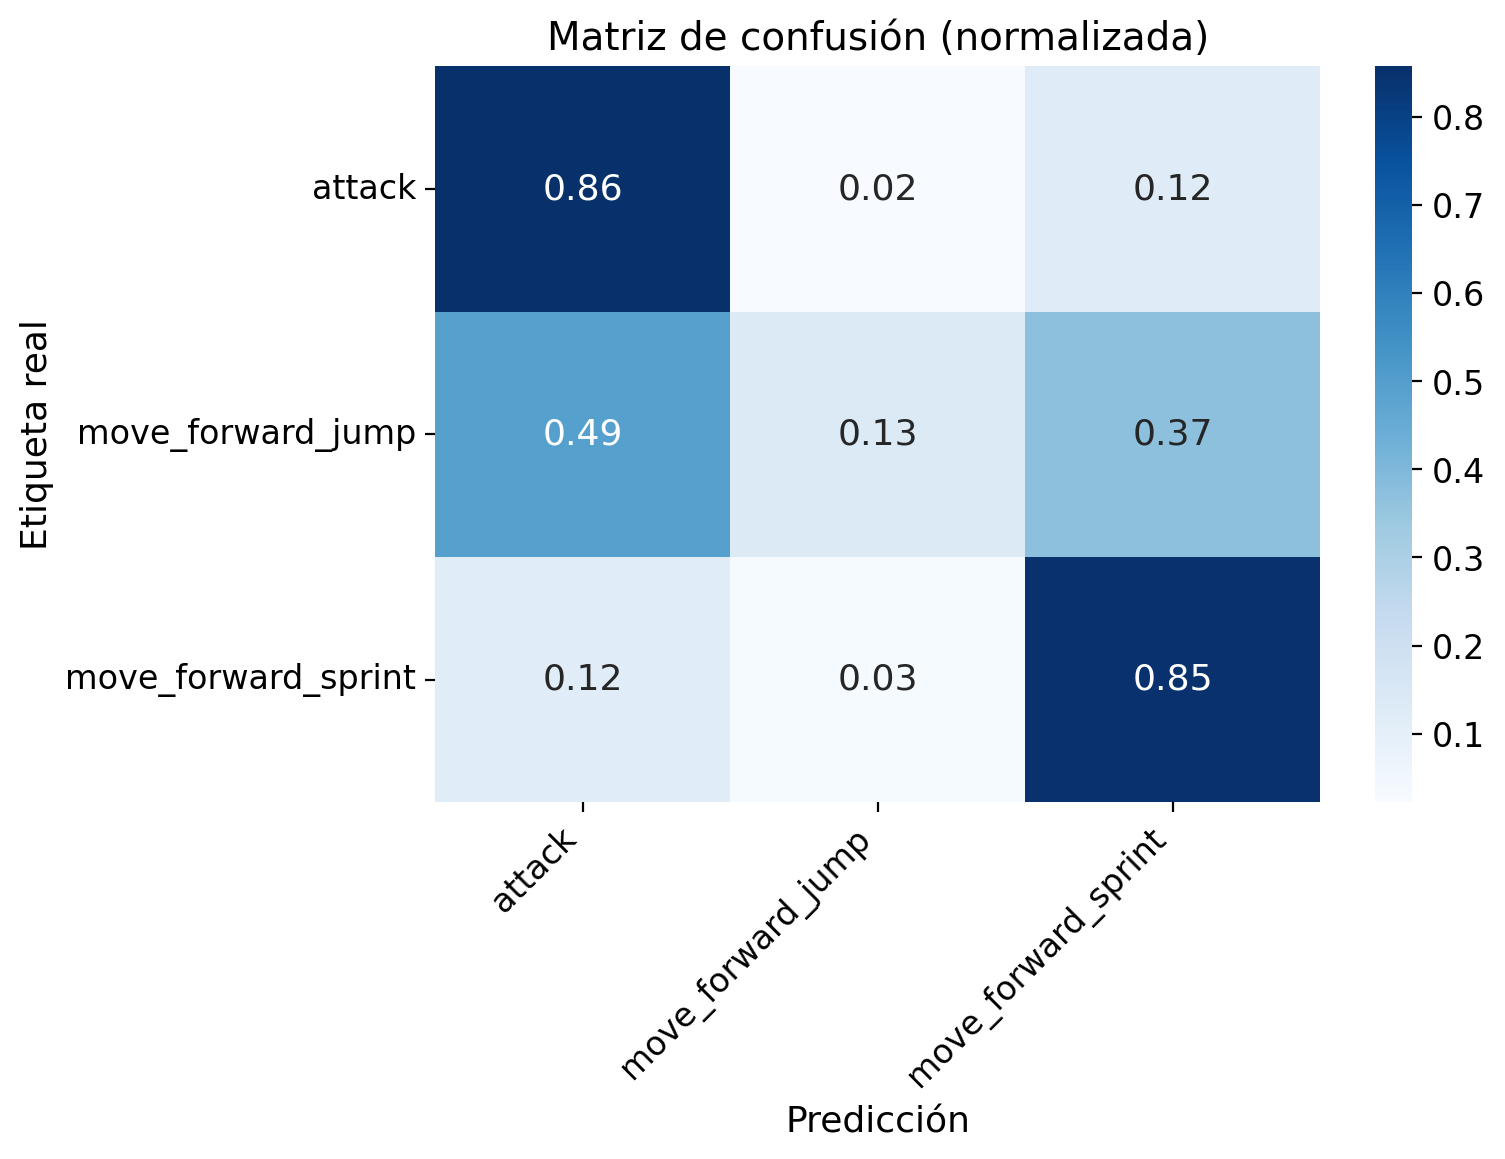
\includegraphics[width=0.7\textwidth]{imaxes/07_il/il_confusion_matrix.png}
  \caption[Matriz de confusión del agente de imitación]{Matriz de confusión sobre el
  conjunto de validación. Los errores se concentran entre las dos acciones de avance;
  la acción dominante \textit{attack} se clasifica con alta fiabilidad.}
  \label{fig:il-confusion}
\end{figure}

En las imágenes del visor (véase el Apéndice~\ref{apx:frame}), el agente simbólico podría realizar ambas acciones de movimiento:
tanto \textit{move\_forward\_sprint} como \textit{move\_forward\_jump} para llegar al mismo resultado. 
Cabe mencionar que la división de estas dos acciones es deliberada: si solo usásemos las acciones de \textit{jump} y
\textit{move\_forward\_sprint}, el agente sería incapaz de sobrepasar bloques, ya que la acción de \textit{jump}
no realiza movimiento horizontal, solo vertical.
Lo más importante es que, si reducimos las acciones a atacar y moverse, observamos que el agente sí que aprende los comportamientos de
acercarse al tronco y atacarlo (Figura~\ref{fig:il_matriz_binaria}, página~\pageref{fig:il_matriz_binaria}). La confusión que podría generarse en este escenario binario
viene dada por una razón similar: las acciones de movimiento y de ataque tienen imágenes bastante similares, diferenciándose
principalmente por la distancia al tronco y la posición de la cámara.

\begin{figure}[htbp]
  \centering
  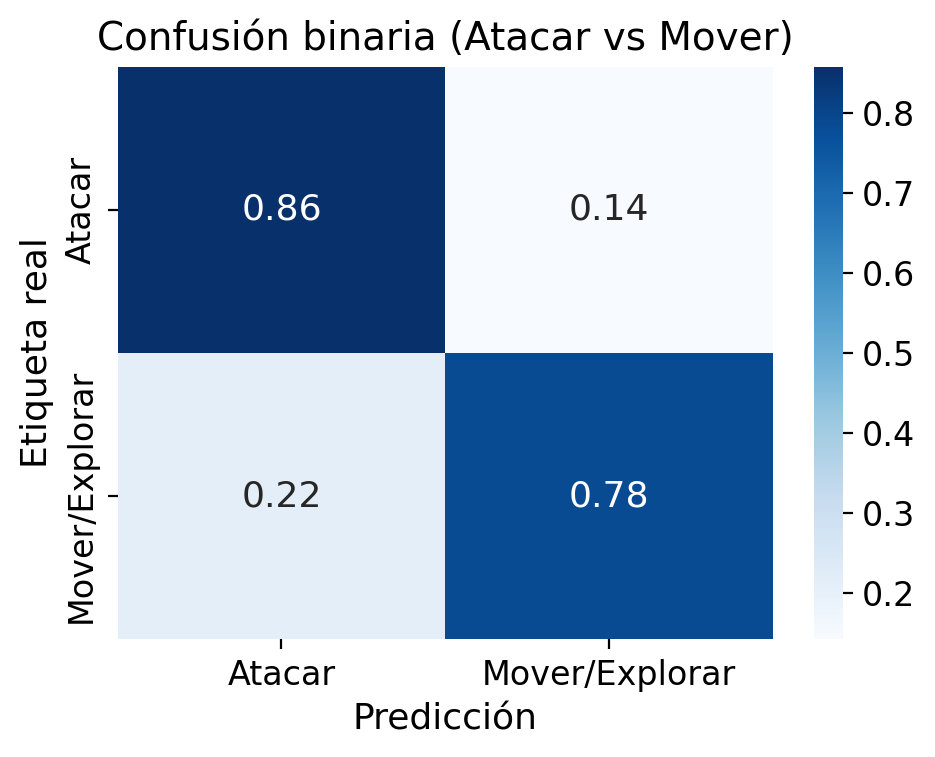
\includegraphics[width=0.5\textwidth]{imaxes/07_il/il_matriz_binaria.png}
  \caption[Matriz de confusión binaria (atacar vs movimiento)]{Matriz de confusión sobre
  el conjunto de validación colapsando las dos acciones de avance
  (\textit{move\_forward\_sprint} y \textit{move\_forward\_jump}) en una única clase
  \textbf{Mover/Explorar} frente a \textbf{Atacar}. Al eliminar la ambigüedad entre las
  dos acciones de avance, la precisión sube al \qty{83.0}{\percent} (frente al \qty{77.3}{\percent} de las
  tres clases): el agente distingue con fiabilidad cuándo acercarse al tronco
  (\qty{78}{\percent}) de cuándo talarlo (\qty{86}{\percent}).}
  \label{fig:il_matriz_binaria}
\end{figure}

\section{Servidor de inferencia}
Siguiendo la arquitectura de tres capas del Capítulo~\ref{chap:arquitectura}, el
modelo entrenado (\textit{Python}) y el control del agente (\textit{Node.js}) se comunican
por \acrshort{http}: un servidor de inferencia expone el \gls{endpoint} \textit{POST /predict},
que recibe la imagen del visor y el estado del agente y responde con la acción predicha, su
confianza y el desplazamiento de cámara desnormalizado (en radianes).

Sobre esta comunicación, el \textit{ILAgent} (capa de agentes) ejecuta un bucle
\textit{percepción} $\rightarrow$ \textit{decisión} $\rightarrow$ \textit{acción}
(Figura~\ref{fig:il-loop}, página~\pageref{fig:il-loop}): captura el
\textit{prismarine-viewer} con \textit{Puppeteer}, lo envía al servidor junto con el estado
actual y ejecuta en \textit{Mineflayer} la acción que recibe.


\begin{figure}[htbp]
  \centering
  \begin{tikzpicture}[
    font=\footnotesize, >=Latex, node distance=6mm,
    proc/.style ={draw, rounded corners, align=center, minimum width=32mm, minimum height=11mm},
    py/.style   ={proc, fill=udcpink!8},
    js/.style   ={proc, fill=udcgray!8},
    lbl/.style  ={font=\scriptsize, align=center, inner sep=2pt, fill=white},
    sw/.style   ={draw, rounded corners=1pt, minimum width=4mm, minimum height=3mm},
  ]
    % Columna 1 - izq
    \node[js] (cap)   {Captura del visor\\\scriptsize \textit{Puppeteer}};
    \node[js] (state) [below=6mm of cap] {Estado del agente};

    \path (cap.east) -- (state.east) coordinate[midway] (mid_east);

    % Columna 2 - der
    \node[py] (srv)   [right=16mm of mid_east] {Servidor de inferencia\\\scriptsize \textit{POST /predict}};
    \node[py] (model) [below=10mm of srv] {Modelo doble cabeza\\\scriptsize (acción $+\;\Delta$cámara)};
    \node[js] (post)  [below=10mm of model] {Post-proceso\\\scriptsize umbral $\cdot$ zona muerta\\\scriptsize \textit{pitch decay}};

    % Vuelta a Columna 1 
    \node[js] (exec)  at (cap |- post) {Ejecutar acción\\\scriptsize \textit{Mineflayer}};

    % Conexiones de ida
    \draw[->, rounded corners=2pt] (cap.east) -- ++(8mm,0) |- ($(srv.west)+(0,2mm)$);
    \draw[->, rounded corners=2pt] (state.east) -- ++(8mm,0) |- ($(srv.west)+(0,-2mm)$);
    \draw[->] (srv.south) -- (model.north);
    \draw[->] (model.south) -- node[lbl]{predicción} (post.north);
    \draw[->] (post.west) -- (exec.east);

    % Bucle 
    \coordinate (loop_turn) at ($(exec.west) + (-12mm, 0)$);
    \draw[->, thick, rounded corners=4pt] (exec.west) -- (loop_turn) |- (cap.west);
    \draw[->, thick] (loop_turn |- state.west) -- (state.west); % Ramificación al estado

    % Leyenda 
    \node[sw, fill=udcgray!8] (ljs) at ($(exec.south west)+(2mm,-12mm)$) {};
    \node[lbl, right=1mm of ljs, anchor=west, fill=none] {\textit{Node.js} (capa de agentes)};
    \node[sw, fill=udcpink!8] (lpy) [right=34mm of ljs] {};
    \node[lbl, right=1mm of lpy, anchor=west, fill=none] {\textit{Python} (capa de decisión)};
  \end{tikzpicture}
  \caption[Bucle de inferencia del agente de imitación]{Bucle
  \textit{percepción\,$\rightarrow$\,decisión\,$\rightarrow$\,acción} del
  \textit{ILAgent}. La captura del visor y el vector de estado (\textit{Node.js}) se envían
  al servidor de inferencia (\textit{Python}), que devuelve la acción discreta y el
  desplazamiento de cámara; la predicción se post-procesa (umbral de confianza, zona
  muerta de cámara y decaimiento de \textit{pitch}) y se ejecuta en \textit{Mineflayer},
  cerrando el bucle en tiempo real.}
  \label{fig:il-loop}
\end{figure}

Se aplican tres matices a la evaluación para adaptar la política a la ejecución en tiempo real:
\begin{itemize}
  \item \textbf{Umbral de confianza}: solo se cambia de acción si la confianza de la
  nueva supera un umbral (\num{0.7}); en caso contrario se mantiene la acción anterior.
  Esto reduce la ambigüedad entre estados similares, produciendo un comportamiento
  más estable.
  \item \textbf{Zona muerta de cámara}: los desplazamientos de cámara por debajo de
  $\sim\qty{0.01}{\radian}$ se ignoran por considerarse ruido.
  \item \textbf{Decaimiento del \textit{pitch}}: tras aplicar el delta, el \textit{pitch}
  se reduce para contrarrestar la acumulación de pequeños errores
  que, sin corrección, provocarían que el agente apuntara la cámara al suelo o al cielo.
\end{itemize}

Además, la acción discreta \textit{attack} se ejecuta como
la primitiva de minar del \gls{htn} (una vez comenzada se realiza hasta romper el bloque), 
garantizando que la acción de atacar complete la tala del bloque, igual que lo haría el experto.

\section{Resultados de la iteración}
El agente de imitación se evalúa en el mismo entorno y
bajo la misma métrica común que el resto de técnicas (recoger al menos $k$ troncos, con $k=\num{5}$).
Esto permite comparar al aprendiz con su tutor en igualdad de condiciones. En la Figura~\ref{fig:il-action-dist} 
(página~\pageref{fig:il-action-dist}) se observa la distribución de acciones del agente de imitación.

\begin{figure}[htbp]
  \centering
  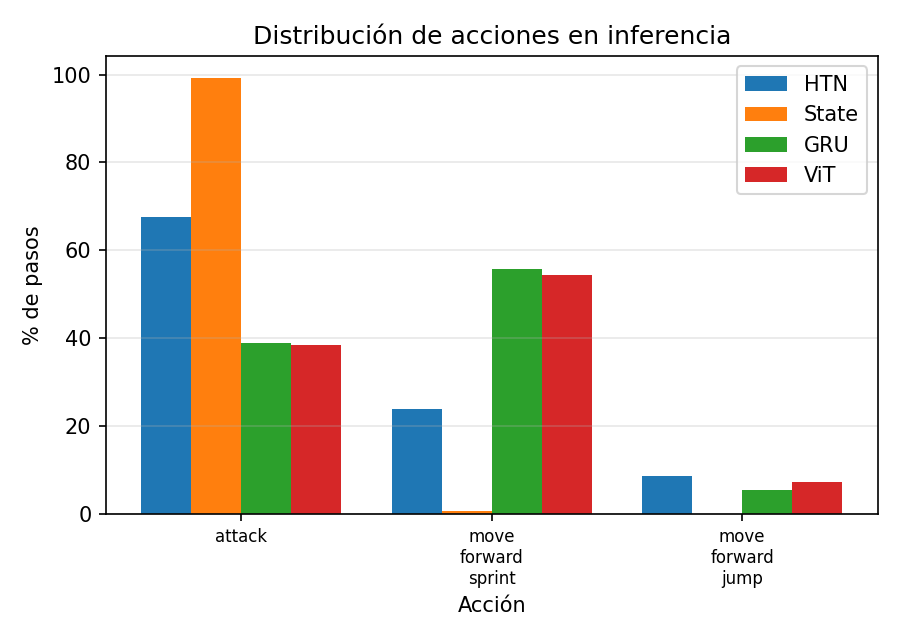
\includegraphics[width=0.8\textwidth]{imaxes/07_il/il_action_dist.png}
  \caption[Distribución de acciones del agente de imitación por técnica]{Distribución de acciones del
  agente de imitación por técnica. La \gls{gru} y la \gls{vit} presentan una distribución de acciones
  más similar a la del experto (\gls{htn}), mientras que la \gls{convlstm} y la variante solo-estado apenas se mueven 
  y atacan en casi todos los \textit{frames}.}
  \label{fig:il-action-dist}
\end{figure}

En ella podemos apreciar que las dos arquitecturas con una distribución de acciones más similar a la del
experto son la \gls{gru} y la \gls{vit}, con distribuciones similares entre sí. Las otras dos aproximaciones,
la \gls{convlstm} y la variante solo-estado, presentan una distribución de acciones muy característica:
ambas realizan la acción de atacar en casi todos los \textit{frames} y apenas se mueven. Esto indica, como
se menciona en la Sección~\ref{sec:solo-estado} (página~\pageref{sec:solo-estado}), que la información visual obtenida del extractor es
la que permite al agente aprender a moverse y atacar. Esto queda confirmado al ver el rendimiento
de la \gls{convlstm} en la Tabla~\ref{tab:il-eval} (página~\pageref{tab:il-eval}), ya que su extractor visual
es una \gls{cnn} simple, obteniendo un éxito inferior
incluso al de la variante solo-estado, que no tiene información visual. Esto indica que la \gls{cnn} no es
capaz de extraer correctamente la información de la imagen. E incluso puede llegar a reducir el funcionamiento del modelo.

\begin{table}[htbp]
  \centering
  \small
  \resizebox{\textwidth}{!}{
  \rowcolors{3}{white}{udcgray!25}
  \resizebox{\textwidth}{!}{
  \begin{tabular}{l|r|r|rrr|rrr}
  \rowcolor{udcpink!25}
   & & & \multicolumn{3}{c|}{\textbf{Troncos}} & \multicolumn{3}{c}{\textbf{Tiempo (s)}} \\
  \rowcolor{udcpink!25}
  \textbf{Técnica} & \textbf{Eps.} & \textbf{Éxito (\%)} & $\boldsymbol{\mu}$ & \textbf{$\tilde{x}$} & $\boldsymbol{\sigma}$ & $\boldsymbol{\mu}$ & \textbf{$\tilde{x}$} & $\boldsymbol{\sigma}$ \\\hline
  HTN & \num{50} & \num{100.0} & \num{6.00} & \num{6.00} & \num{0.00} & \num{26.7} & \num{26.4} & \num{1.1} \\
  IL-STATE & \num{50} & \num{4.0} & \num{0.54} & \num{0.00} & \num{1.25} & \num{195.8} & \num{202.1} & \num{34.1} \\
  IL-GRU & \num{50} & \num{52.0} & \num{3.84} & \num{5.00} & \num{1.82} & \num{156.2} & \num{203.4} & \num{67.3} \\
  IL-CONV & \num{50} & \num{0.0} & \num{0.08} & \num{0.00} & \num{0.27} & \num{203.0} & \num{202.1} & \num{3.3} \\
  IL-VIT & \num{32} & \num{37.5} & \num{3.00} & \num{3.50} & \num{1.90} & \num{169.4} & \num{208.6} & \num{67.9} \\
  \end{tabular}
  }
  }
  \caption[Evaluación de las técnicas de imitación]{Evaluación de las técnicas de imitación bajo la métrica común recoger $k=\num{5}$ troncos.
  Troncos y tiempo por episodio: media ($\mu$), mediana (\textbf{$\tilde{x}$}) y desviación típica ($\sigma$).}
  \label{tab:il-eval}
\end{table}


\subsection{Análisis de resultados}
\label{sec:il-sin-exploracion}
Durante el proceso de evaluación se encontró una limitación del modelo de imitación
que no se refleja en los resultados mencionados hasta ahora. El agente es capaz de
aprender la tarea de talar un árbol visible; es decir, cuando hay un tronco dentro del campo de
visión y al alcance, se orienta hacia él, se acerca y lo ataca correctamente.

Sin embargo, el agente \textbf{no presenta exploración}: es incapaz de buscar consistentemente
un árbol que esté lejos y acercarse a él. En escenarios donde el árbol no está en el campo de visión inicial,
el agente tiene un rendimiento considerablemente peor.

La causa de esta separación viene de las demostraciones generadas por el experto. Al 
localizar los troncos con la información de la \acrshort{api} y navegar de forma
óptima con el \gls{pathfinder}, nunca realiza la tarea de exploración ni realiza una búsqueda 
visual. En consecuencia, el \textit{dataset} no contiene
comportamiento exploratorio real: el aprendiz solo ha visto cómo talar
un árbol que tiene enfrente, pero no cómo encontrarlo mediante exploración. 
Teniendo esto en cuenta, todas las evaluaciones de las técnicas se realizan en un entorno
con árboles al alcance del campo de visión inicial.

\subsection{Alcance del agente de imitación}
La falta de exploración descrita es un síntoma de un problema más general de la imitación.
Cuando el agente aprendido se desvía de la trayectoria del experto, visita estados poco
representados en las demostraciones, donde la política no es tan precisa. Este problema se
denomina \textit{\gls{distribution-shift}}~\cite{DBLP:journals/jmlr/RossGB11}: los errores se
acumulan a lo largo del episodio porque el experto no enseñó cómo salir de las situaciones
que provoca el propio aprendiz.

Esta limitación es precisamente lo que motiva la Iteración~III, desarrollada en el Capítulo~\ref{chap:iter3}.
El aprendizaje por refuerzo permite que el agente \emph{explore} y corrija sus propios 
errores mediante la recompensa, en lugar de depender de un experto que cubra todas las posibilidades. 
Además, la política de imitación puede servir para inicializar el agente de refuerzo
mediante \gls{bc}, como se explora en el Capítulo~\ref{chap:conclusions}.